\documentclass[border=5pt]{standalone}
\usepackage{mathtools}
\DeclarePairedDelimiter\abs{\lvert}{\rvert}%
\DeclarePairedDelimiter\norm{\lVert}{\rVert}%
\usepackage{pgfplots}

\pgfkeys{/pgfplots/Delta Style/.style={
    % scale only axis,
    % grid=major,
    axis equal,
    grid style={dashed, gray!30}, %Uncomment these lines for no grid
    axis lines=middle,
    inner axis line style={=stealth}, %Arrow type
    ultra thick,
    xlabel={\large $x$},
    ylabel={\large $y$},
    cycle list = {black,black!70,black!40,black!10} %Plot colors cycle in grayscale
  }}

\begin{document}
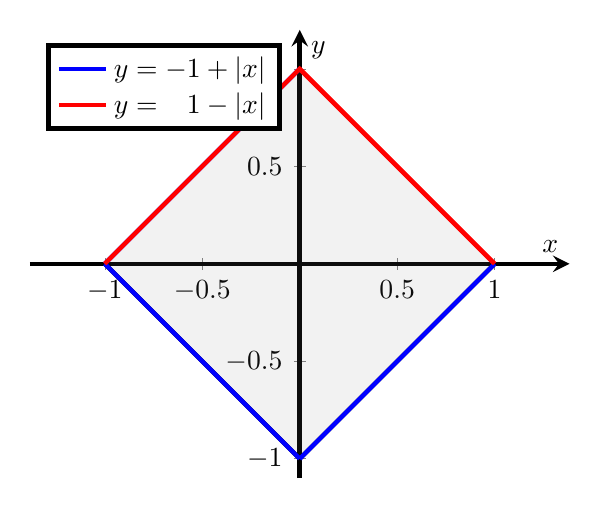
\begin{tikzpicture}
  \begin{axis}[ Delta Style, xlabel = {$x$}, ylabel = {$y$},
    domain=-1:1,ymin=-1.1,ymax=1.2, legend pos=north west ]
    % Here the blue parabloa is defined

    \addplot [blue, fill = gray, fill opacity = 0.1, domain = -1:0, ] {1+x};
    \addlegendentry{$y=-1 + \abs{x}$};
 
    \addplot [red, fill = gray, fill opacity = 0.1, domain = 0:1, ] {1-x};
    
    \addplot [fill = gray, fill opacity = 0.1, ] {-1+abs(x)};
    
    \addplot [blue, fill = gray, fill opacity = 0.1, domain = 0:1, ] {-1+x};
 
    \addplot [blue, fill = gray, fill opacity = 0.1, domain = -1:0, ] {-1-x};
    \addlegendentry{$y=\phantom{-}1 - \abs{x}$};
    
    \addplot [red, fill = gray, fill opacity = 0.1, ] {1-abs(x)};

  \end{axis}
\end{tikzpicture}
\end{document}
